\documentclass[12pt, a4paper]{article}

\usepackage{amsmath}
\usepackage{amsfonts}
\usepackage{amssymb}
\usepackage{graphicx}
\usepackage{float}
\usepackage{listings}
\usepackage{rotating}
\usepackage{tikz}
\usepackage{verbatim}
\pdfgentounicode=1
\pdfmapline{+cyberb@Unicode@  <cyberbit.ttf}

\begin{document}

\title{PBMath}
\author{P. Baillehache}
\date{\today}
\maketitle

\tableofcontents

\section*{Introduction}

PBMath is C library providing mathematical structures and functions.\\ 

The \begin{ttfamily}VecFloat\end{ttfamily} structure and its functions can be used to manipulate vectors of float values.\\

The \begin{ttfamily}Gauss\end{ttfamily} structure and its functions can be used to get values of the Gauss function and random values distributed accordingly with a Gauss distribution.\\

The \begin{ttfamily}Smoother\end{ttfamily} functions can be used to get values of the SmoothStep and SmootherStep functions.\\

\section{Definitions}

\subsection{Angle between two vectors}

The problem is as follow: given two vectors $\vec{V}$ and $\vec{W}$ not null, how to calculate the angle $\theta$ from $\vec{V}$ to $\vec{W}$.\\

Let's call $M$ the rotation matrix: $M\vec{V}=\vec{W}$, and the components of $M$ as follow:
\begin{equation}
M=\left[
\begin{array}{cc}
Ma&Mb\\
Mc&Md\\
\end{array}
\right]=\left[
\begin{array}{cc}
cos(\theta)&-sin(\theta)\\
sin(\theta)&cos(\theta)\\
\end{array}
\right]
\end{equation}
Then, $M\vec{V}=\vec{W}$ can be written has 
\begin{equation}
\left\lbrace
\begin{array}{l}
W_x = M_aV_x+M_bV_y\\
W_y = M_cV_x+M_dV_y\\
\end{array}
\right.
\end{equation}
Equivalent to
\begin{equation}
\left\lbrace
\begin{array}{l}
W_x = M_aV_x+M_bV_y\\
W_y = -M_bV_x+M_aV_y\\
\end{array}
\right.
\end{equation}
where $M_a=cos(\theta)$ and $M_b=-sin(\theta)$.\\
If $Vx\neq0.0$, we can write
\begin{equation}
\left\lbrace
\begin{array}{l}
M_b = \frac{M_aV_y-W_y}{V_x}\\
M_a = \frac{W_x+W_yV_y/V_x}{V_x+V_y^2/V_x}\\
\end{array}
\right.
\end{equation}
Or, if $Vx=0.0$, we can write
\begin{equation}
\left\lbrace
\begin{array}{l}
Ma = \frac{W_y+M_bV_x}{V_y}\\
Mb = \frac{W_x-W_yV_x/V_y}{V_y+V_x^2/V_y}\\
\end{array}
\right.
\end{equation}
Then we have $\theta=\pm cos^{-1}(M_a)$ where the sign can be determined by verifying that the sign of $sin(\theta)$ matches the sign of $-M_b$: if $sin(cos^{-1}(M_a))*M_b > 0.0$ then multiply $\theta=-cos^{-1}(M_a)$ else $\theta=cos^{-1}(M_a)$.

\subsection{Shapoid}

\subsubsection{Definition}

A Shapoid is a geometry defined by its dimension $D\in\mathbb{N^*_+}$ equals to the number of dimensions of the space it exists in, its position $\overrightarrow{P}$, and its axis $(\overrightarrow{A_0},\overrightarrow{A_1},...,\overrightarrow{A_{D-1}})$. $A_i$ and $P$ are vectors of dimension $D$. In what follows I'll use $I$ as notation for the interval $[0,D-1]$ for simplification.\\

Shapoids are classified in three groups: Facoid, Pyramidoid and Spheroid. The volume of a Shapoid is defined by, for a Facoid: 
\begin{equation}
\left\lbrace \sum_{i\in I}v_i\overrightarrow{A_i}+\overrightarrow{P}\right\rbrace ,v_i\in[0.0,1.0]
\end{equation}
for a Pyramidoid:
\begin{equation}
\left\lbrace \sum_{i\in I}v_i\overrightarrow{A_i}+\overrightarrow{P}\right\rbrace ,v_i\in[0.0,1.0], \sum_{i\in I}v_i\le1.0
\end{equation}
and for a Spheroid:
\begin{equation}
\begin{array}{rl}
\left\lbrace \sum_{i\in I}(v_i-0.5)\overrightarrow{A_i}+\overrightarrow{P}\right\rbrace ,&\\
v_i\in[0.0,1.0],&\sum_{i\in I}(v_i-0.5)^2\le0.25
\end{array}
\end{equation}

\subsubsection{Transformation}

A translation of a Shapoid by $\overrightarrow{T}$ is obtained as follow:\\
\begin{equation}
\left(\overrightarrow{P},\left\lbrace\overrightarrow{A_i}\right\rbrace_{i\in I}\right)\mapsto\left(\overrightarrow{P}+\overrightarrow{T},\left\lbrace\overrightarrow{A_i}\right\rbrace_{i\in I}\right)
\end{equation} 
A scale of a Shapoid by $\overrightarrow{S}$ is obtained as follow:\\
\begin{equation}
\left(\overrightarrow{P},\left\lbrace\overrightarrow{A_i}\right\rbrace_{i\in I}\right)\mapsto\left( \overrightarrow{P},\left\lbrace\overrightarrow{A'_i}\right\rbrace_{i\in I}\right)
\end{equation} 
where
\begin{equation}
\overrightarrow{A'_i}=S_i\overrightarrow{A_i}
\end{equation}
For Shapoid whose dimension $D$ is equal to 2, a rotation by angle $\theta$ is obtained as follow:\\
\begin{equation}
\left(\overrightarrow{P},\overrightarrow{A_0},\overrightarrow{A_1}\right)\mapsto\left(\overrightarrow{P},\overrightarrow{A'_0},\overrightarrow{A'_1}\right)
\end{equation} 
where
\begin{equation}
\overrightarrow{A'_i}=\left[
\begin{array}{cc}
cos\theta&-sin\theta\\
sin\theta&cos\theta\\
\end{array}
\right]
\overrightarrow{A_i}
\end{equation}

\subsubsection{Shapoid's coordinate system}

The Shapoid's coordinate system is the system having $\overrightarrow{P}$ as origin and $\overrightarrow{A_i}$ as axis. One can change from the Shapoid's coordinate system ($\overrightarrow{X^S}$) to the standard coordinate system ($\overrightarrow{X}$) as follow:\\
\begin{equation}
\overrightarrow{X}=\left[\left(\overrightarrow{A_0}\right)\left(\overrightarrow{A_1}\right)...\left(\overrightarrow{A_{D-1}}\right)\right]\overrightarrow{X^S}+\overrightarrow{P}
\end{equation}
and reciprocally, from the standard coordinate system to the Shapoid's coordinate system:\\
\begin{equation}
\overrightarrow{X^S}=\left[\left(\overrightarrow{A_0}\right)\left(\overrightarrow{A_1}\right)...\left(\overrightarrow{A_{D-1}}\right)\right]^{-1}\left(\overrightarrow{X}-\overrightarrow{P}\right)
\end{equation}

\subsubsection{Insideness}

$\overrightarrow{X}$ is inside the Shapoid $S$ if, for a Facoid:\\
\begin{equation}
\forall i\in I,0.0\le X_i^S\le1.0
\end{equation}
for a Pyramidoid:\\
\begin{equation}
\left\lbrace\begin{array}{l}
\forall i\in I,0.0\le X_i^S\le1.0\\
\sum_{i\in I}X_i^S\le1.0
\end{array}\right.
\end{equation}
for a Spheroid:\\
\begin{equation}
\left|\left|\overrightarrow{X^S}\right|\right|\le0.5
\end{equation}

\subsubsection{Bounding box}

A bounding box of a Shapoid is a Facoid whose axis are colinear to axis of the standard coordinate system, and including the Shapoid in its volume. While the smallest possible bounding box can be easily obtained for Facoid and Pyramidoid, it's more complicate for Spheroid. Then we will consider for the Spheroid the bounding box of the equivalent Facoid $\left(\overrightarrow{P}-\sum_{i\in I}\left(0.5*\overrightarrow{A_i}\right),\left\lbrace\overrightarrow{A_i}\right\rbrace_{i\in I}\right)$ which gives the smallest bounding box when axis of the Spheroid are colinear to axis of the standard coordinate system and a bounding box slightly too large when not colinear.\\
The bounding box is defined as follow, for a Facoid:\\
\begin{equation}
\left(\overrightarrow{P'},\left\lbrace\overrightarrow{A'_i}\right\rbrace_{i\in I}\right)
\end{equation}
where\\
\begin{equation}
\left\lbrace
\begin{array}{l}
P'_i=P_i+\sum_{j\in I^-}A_{ji}\\
A'_{ij}=0.0,i\neq j\\
A'_{ij}=\sum_{k\in I^+}A_{kj}-\sum_{k\in I^-}A_{kj},i=j\\
\end{array}
\right.
\end{equation}
and, $I^+$ and $I^-$ are the subsets of $I$ such as $\forall j\in I^+,A_{ij}\ge 0.0$ and $\forall j\in I^-,A_{ij}<0.0$.\\

for a Pyramidoid:\\
\begin{equation}
\left(\overrightarrow{P'},\left\lbrace\overrightarrow{A'_i}\right\rbrace_{i\in I}\right)
\end{equation}
where\\
\begin{equation}
\left\lbrace
\begin{array}{l}
P'_i=P_i+Min\left(Min_{j\in I}(A_{ji}),0.0\right)\\
A'_{ij}=0.0,i\neq j\\
A'_{ij}=Max_{k\in I}(A_{kj})-Min\left(Min_{k\in I}(A_{kj}),0.0\right),i=j\\
\end{array}
\right.
\end{equation}


\subsubsection{Depth and Center}

Depth $\mathbf{D}_S(\overrightarrow{X})$ of position $\overrightarrow{X}$ a Shapoid $S$ is a value ranging from 0.0 if $\overrightarrow{X}$ is on the surface of the Shapoid, to 1.0 if $\overrightarrow{X}$ is at the farthest location from the surface inside the Shapoid. Depth is by definition equal to 0.0 if $\overrightarrow{X}$ is outside the Shapoid. Depth is continuous and derivable on the volume of the Shapoid. It is defined by, for a Facoid:\\
\begin{equation}
\mathbf{D}_S(\overrightarrow{X})=\prod_{i\in I}\left(1.0-4.0*(0.5-X^S_i)^2\right)
\end{equation}
for a Pyramidoid:\\
\begin{equation}
\mathbf{D}_S(\overrightarrow{X})=\prod_{i\in I}\left(1.0-4.0*\left(0.5-\frac{X^S_i}{1.0-\sum_{j\in I-\lbrace i\rbrace}X^S_j}\right)^2\right)
\end{equation}
and for a Spheroid:\\
\begin{equation}
\mathbf{D}_S(\overrightarrow{X})=1.0-2.0*\left|\left|\overrightarrow{X^S}\right|\right|
\end{equation}
The maximum depth is obtained at $\overrightarrow{C}$ such as, for a Facoid:\\
\begin{equation}
\forall i\in I,C_i^S=0.5
\end{equation}
for a Pyramidoid:\\
\begin{equation}
\forall i\in I,C_i^S=\frac{1}{D+1}
\end{equation}
for a Spheroid:\\
\begin{equation}
\forall i\in I,C_i^S=0.0
\end{equation}
$\overrightarrow{C}$ is called the center of the Shapoid.

\section{Interface}

\begin{scriptsize}
\begin{ttfamily}
\verbatiminput{../pbmath.h}
\end{ttfamily}
\end{scriptsize}

\section{Code}

\begin{scriptsize}
\begin{ttfamily}
\verbatiminput{../pbmath.c}
\end{ttfamily}
\end{scriptsize}

\section{Makefile}

\begin{scriptsize}
\begin{ttfamily}
\verbatiminput{../Makefile}
\end{ttfamily}
\end{scriptsize}

\section{Usage}

\begin{scriptsize}
\begin{ttfamily}
\verbatiminput{../main.c}
\end{ttfamily}
\end{scriptsize}

Output:\\
\begin{scriptsize}
\begin{ttfamily}
\verbatiminput{../output.txt}
\end{ttfamily}
\end{scriptsize}

vecshort.txt:\\
\begin{scriptsize}
\begin{ttfamily}
\verbatiminput{../vecshort.txt}
\end{ttfamily}
\end{scriptsize}

vecfloat.txt:\\
\begin{scriptsize}
\begin{ttfamily}
\verbatiminput{../vecfloat.txt}
\end{ttfamily}
\end{scriptsize}

matfloat.txt:\\
\begin{scriptsize}
\begin{ttfamily}
\verbatiminput{../matfloat.txt}
\end{ttfamily}
\end{scriptsize}

smoother functions:\\
\begin{center}
\begin{figure}[H]
\centering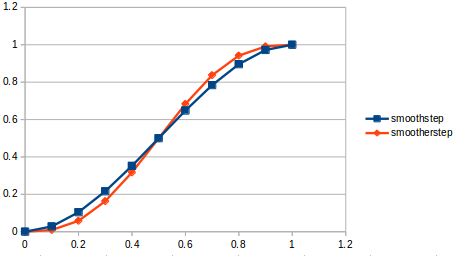
\includegraphics[width=6cm]{./smoother.png}\\
\end{figure}
\end{center}

gauss function (mean:0.0, sigma:1.0):\\
\begin{center}
\begin{figure}[H]
\centering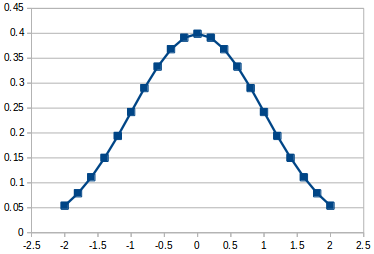
\includegraphics[width=6cm]{./gauss.png}\\
\end{figure}
\end{center}

gauss rand function (mean:1.0, sigma:0.5):\\
\begin{center}
\begin{figure}[H]
\centering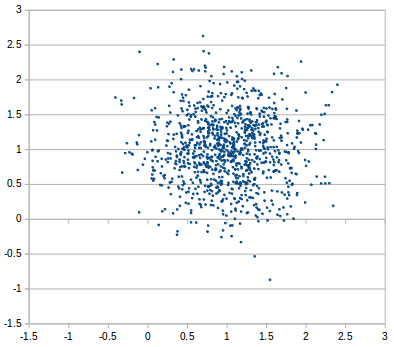
\includegraphics[width=6cm]{./gaussrnd.png}\\
\end{figure}
\end{center}

\end{document}


